% Titre de la premiere partie
\section{\texttt{git}, GitHub et GitHub Classroom}

%%%%%%%%%%%%%%%%%%%%%%%%%%%%%%%%%%%%%%%%%%%%%%%%
% Diapo Git
%%%%%%%%%%%%%%%%%%%%%%%%%%%%%%%%%%%%%%%%%%%%%%%%
\begin{frame}
\frametitle{\texttt{git}}
\framesubtitle{Logiciel de gestion de versions décentralisé}

\begin{center}
	
\includegraphics[height=0.8\textheight]{figures/Strips-_Old-650-final1.jpg}
\end{center}

\end{frame}

%%%%%%%%%%%%%%%%%%%%%%%%%%%%%%%%%%%%%%%%%%%%%%%%
% Diapo Git
%%%%%%%%%%%%%%%%%%%%%%%%%%%%%%%%%%%%%%%%%%%%%%%%
\begin{frame}
\frametitle{\texttt{git}}
\framesubtitle{Logiciel de gestion de versions décentralisé}

\begin{itemize}[<+->]
	\item	 Logiciel libre créé par Linus Torvald en 2005
	\item  Permet des sauvegardes successives mais aussi le travail en parallèle de plusieurs personnes sur un même jeu de fichier (penser aux multiples versions des programmes de simulation en TIPE)
	\item  Accessible par la ligne de commande

	(pratique pour scripter mais pas trop pour les élèves)
	\item  Fonctionne en terme de \ofg{commit} qui rassemble des changements atomiques
	\item 	Permet de multiples actions et un suivi historique des modifications successives.

\end{itemize}

\end{frame}


%%%%%%%%%%%%%%%%%%%%%%%%%%%%%%%%%%%%%%%%%%%%%%%%
% Diapo Github
%%%%%%%%%%%%%%%%%%%%%%%%%%%%%%%%%%%%%%%%%%%%%%%%
\begin{frame}
\frametitle{GitHub}
\framesubtitle{Une interface web pour \texttt{git}}

\begin{itemize}[<+->]
	\item Site web permettant un accès centralisé aux repository git (\url{https://github.com})



	\item Sorte de «facebook» des développeurs

	\item Modèle commercial: repositories publics illimités mais privés payant au-delà de 3 collaborateurs (sauf organisations à visées pédagogiques)

\end{itemize}

\end{frame}


%%%%%%%%%%%%%%%%%%%%%%%%%%%%%%%%%%%%%%%%%%%%%%%%
% Diapo Github
%%%%%%%%%%%%%%%%%%%%%%%%%%%%%%%%%%%%%%%%%%%%%%%%
\begin{frame}
\frametitle{GitHub}
\framesubtitle{Exemple du noyau Linux}

	\begin{center}
			
\includegraphics[width=\linewidth]{figures/github_linux.png}
	\end{center}

\end{frame}

%%%%%%%%%%%%%%%%%%%%%%%%%%%%%%%%%%%%%%%%%%%%%%%%
% Diapo Github
%%%%%%%%%%%%%%%%%%%%%%%%%%%%%%%%%%%%%%%%%%%%%%%%
\begin{frame}
\frametitle{GitHub}
\framesubtitle{Exemple de visualisation de compte}

	\begin{center}
			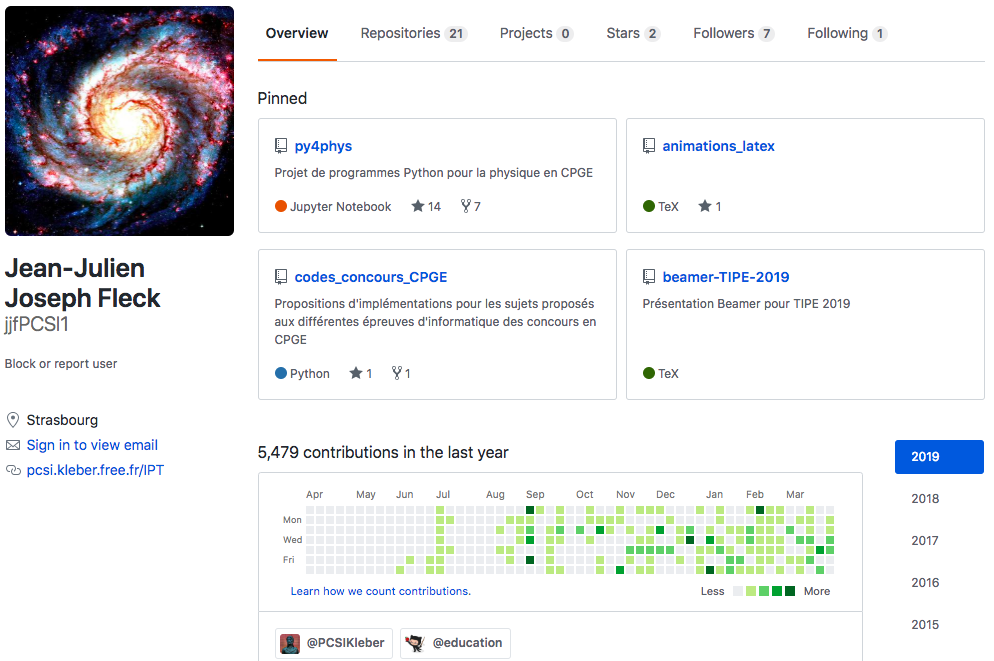
\includegraphics[width=\linewidth]{figures/github_jjfPCSI1.png}
	\end{center}

\end{frame}

%%%%%%%%%%%%%%%%%%%%%%%%%%%%%%%%%%%%%%%%%%%%%%%%
% Diapo github Desktop
%%%%%%%%%%%%%%%%%%%%%%%%%%%%%%%%%%%%%%%%%%%%%%%%
\begin{frame}
	\frametitle{GitHub Desktop}
	\framesubtitle{Interface graphique pour interagir avec GitHub}

	\begin{itemize}[<+->]
		\item Installation facile depuis \url{https://desktop.github.com/}

		\item Permet de rappatrier les repositories depuis GitHub.com sur l'ordinateur en local (\texttt{Clone Repository...})

		\item Permet de faire les commits depuis l'ordinateur local.

		\item Aucune connexion requise pour les commits (on peut bosser dans le train par exemple), il suffit de penser à «pousser» les modifications une fois la connexion rétablie.

		\item Très loin d'utiliser toutes la puissance de \texttt{git} mais justement utile pour ne pas effrayer les élèves

	\end{itemize}

\end{frame}

%%%%%%%%%%%%%%%%%%%%%%%%%%%%%%%%%%%%%%%%%%%%%%%%
% Diapo github Desktop
%%%%%%%%%%%%%%%%%%%%%%%%%%%%%%%%%%%%%%%%%%%%%%%%
\begin{frame}
	\frametitle{GitHub Desktop}
	\framesubtitle{Exemple de visualisation d'historique}

	\begin{center}
		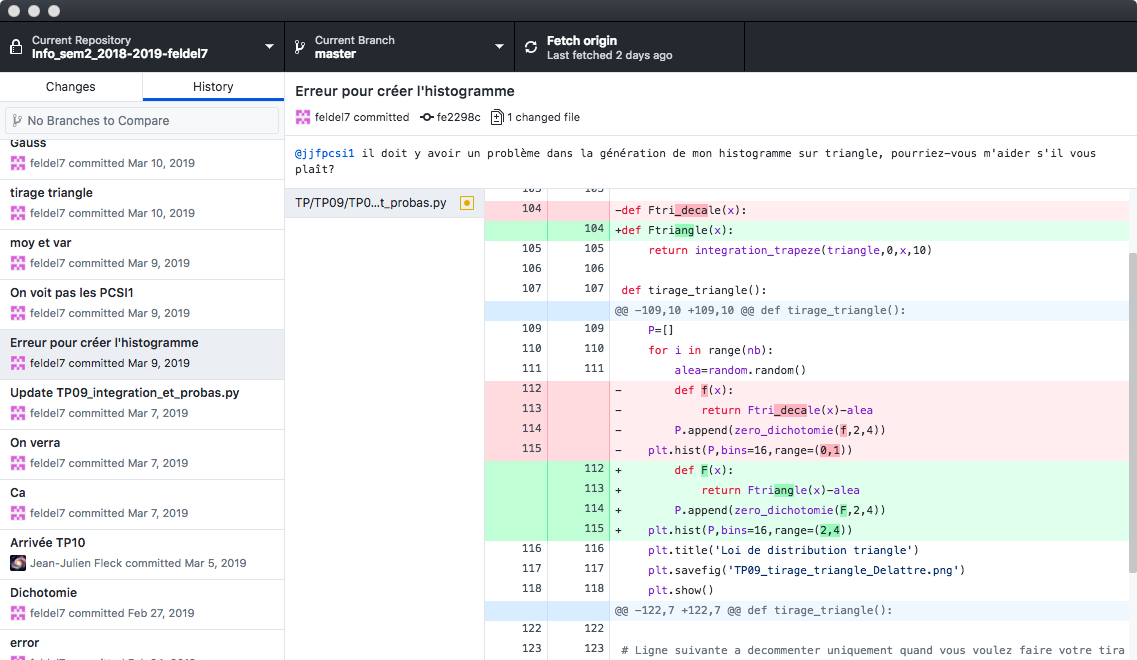
\includegraphics[width=\linewidth]{figures/githubdesktop.png}
	\end{center}

\end{frame}

%%%%%%%%%%%%%%%%%%%%%%%%%%%%%%%%%%%%%%%%%%%%%%%%
% Diapo github Desktop
%%%%%%%%%%%%%%%%%%%%%%%%%%%%%%%%%%%%%%%%%%%%%%%%
\begin{frame}
	\frametitle{GitHub Desktop}
	\framesubtitle{Exemple de visualisation de commit}

	\begin{center}
		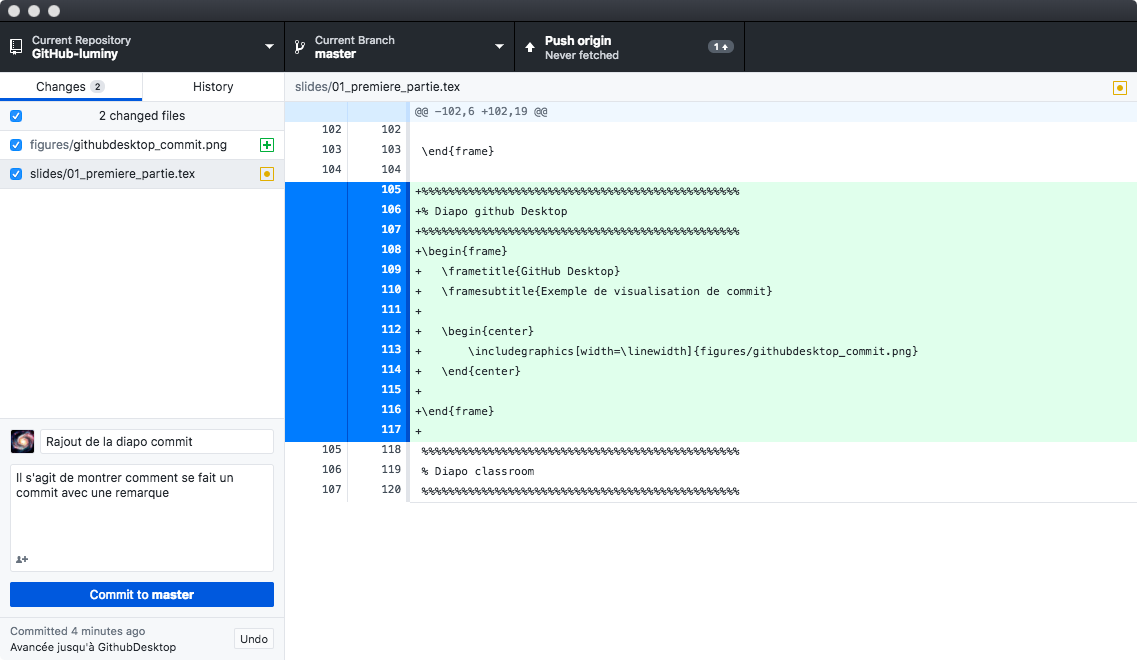
\includegraphics[width=\linewidth]{figures/githubdesktop_commit.png}
	\end{center}

\end{frame}

%%%%%%%%%%%%%%%%%%%%%%%%%%%%%%%%%%%%%%%%%%%%%%%%
% Diapo classroom
%%%%%%%%%%%%%%%%%%%%%%%%%%%%%%%%%%%%%%%%%%%%%%%%
\begin{frame}
	\frametitle{GitHub Classroom \url{https://classroom.github.com/}}
	\framesubtitle{Un service annexe de GitHub}

	\begin{center}
		
\includegraphics[width=\linewidth]{figures/classroom_accueil.png}
	\end{center}

	\begin{itemize}[<+->]
		\item Automatise le processus de création de repositories pour les élèves

		\item Permet de rappatrier les repositories sur l'ordi prof via «classroom assistant» (\url{https://classroom.github.com/assistant})

	\end{itemize}



\end{frame}
